\documentclass{fetch-my-doc}
\usepackage{tabu}
%\usepackage{multirow}
\usepackage{siunitx}
%\usepackage{enumitem}
%\usepackage{fancyvrb}
%\usepackage{breakurl}
%\usepackage{tocloft}
%\usepackage{pdflscape}
%\usepackage{ltxtable}
%\usepackage{filecontents}
\usepackage{onimage}

\usepackage{verbatim}

\sisetup{output-decimal-marker = {,}}

\definecolor{darkgreen}{rgb}{0,.5,0}

\hypersetup{breaklinks,colorlinks=true,citecolor=darkgreen,urlcolor=blue,linkcolor=blue,anchorcolor=blue} %,pdftex=true}

\newcommand{\hypref}[1]{\SaveVerb{myverb}|#1|\hyperlink{#1}{\protect\UseVerb{myverb}}}

\newcommand{\sep}{\begin{center}\noindent\rule{.5\textwidth}{0.5pt}\end{center}}

\newcommand{\rc}{\rowcolor{lightgray!40}}
\newcommand{\cc}{\columncolor{lightgray!40}}

\makeatletter
\newcommand*{\shift}[2]{%
  \settowidth{\@tempdima}{#2}%
  \makebox[\@tempdima]{\hspace*{#1}#2}%
}
\makeatother

% Linebreak nach paragraph
\makeatletter
\renewcommand\paragraph{%
   \@startsection{paragraph}{4}{0mm}%
      {-\baselineskip}%
      {.5\baselineskip}%
      {\normalfont\normalsize\bfseries}}
\makeatother

\def\imagetop#1{\raisebox{2.5em}{\vtop{\null\hbox{#1}}}}

%\renewcommand{\datum}{14.10.2012}
\renewcommand{\datum}{\today}
\renewcommand{\abgabe}{14.07.2014}
\renewcommand{\version}{1.0.0}
	%	Versionierung:
	%	x.y.z
	%	- x hoch bei ?
	%	- y hoch bei größeren Änderungen von ganzen Absätzen.
	%	- z hoch bei kleinen Verbesserungen wie Rechtschreibung, Satzbau, usw.
\renewcommand{\typ}{Dokumentation}
\renewcommand{\titel}{Dokumentation}
\renewcommand{\libdir}{./}
\bibliography{referenzen}

\setcounter{tocdepth}{4}
\setcounter{secnumdepth}{3}

\tikzset{
    image label/.style={
        every node/.style={
            fill=white,
            fill opacity=.5,
            text opacity=1,
            text=orange,
            font=\fontfamily{phv}\selectfont\Large\bfseries}
        }
}

\tikzset{
  state/.style={
         rectangle,
         rounded corners,
         draw=black, very thick,
         minimum height=2em,
         inner sep=2pt,
         text centered,
         },
}

\begin{document}
	\sloppy
	\begin{titlepage}
	\begin{center}
		\vspace*{.7cm}		
		\thispagestyle{FirstPage}
		\textsc{\LARGE \fach}\\
		%\vspace*{.2cm}
		%{\huge Fetch my ball}\\[0.4cm]
		
		\includegraphics[width=0.85\textwidth]{\libdir img/logo1.pdf}\\
		%\textsc{\Large \gruppe}\\[0.5cm]

		% Titel
		\HRule \\[0.4cm]
		{ \huge \bfseries \titel}\\[0.4cm]
		Version \version	\\
		\HRule \\[1.5cm]

		\vfill
		
		% Autoren
		\begin{tabular}{rcl}
			\toprule
			\mgEinsVorname\ \mgEinsNachname		&&	\mgEinsMail	\\
			\mgZweiVorname\ \mgZweiNachname		&&	\mgZweiMail	\\
			\mgDreiVorname\ \mgDreiNachname		&&	\mgDreiMail	\\
			\bottomrule
		\end{tabular}
		
		\vspace{2cm}

		{\large Abgabe: \abgabe}
	\end{center}
	\addtolength{\textheight}{\versch}
\end{titlepage}
	\addtolength{\textheight}{\versch}
	%%%%%%%%%%%%%%%%%%%%%%%%%%%%%%%%%%%%
	% TODOS ENTFERNEN NICHT VERGESSEN! %
	%%%%%%%%%%%%%%%%%%%%%%%%%%%%%%%%%%%%
	%\printtodo
	%%%%%%%%%%%%%%%%%%%%%%%%%%%%%%%%%%%%
	\addtocontents{toc}{\protect\sloppy}
	\tableofcontents
	\clearpage
	
	%\section{Versions- und Änderungsgeschichte}\label{sec:versionsaenderung}
		%\begin{tabularx}{\textwidth}{ccX}
			%\toprule
			%Version			&	Datum						&	Änderungen	\\\midrule
			%1.0.0				&	14.07.2014			&	Erste veröffentlichte Version	\\
			%\bottomrule
		%\end{tabularx}	
		%\clearpage
	
	%\rowcolors*{0}{}{lightgray!40}
	
	%%%%%%%%%% Hier beginnt das Dokument %%%%%%%%%%
	\section{Einführung}\label{sec:Einfuehrung}
		\autor{Hannes, Andreas}
		Im Rahmen der Veranstaltung \textit{Lisp Tutorial} haben wir ein Projekt durchgeführt, um die in den Vorlesungen gewonnenen Kenntnisse in die Praxis umzusetzen.
		
		In dieser Dokumentation wird auf die Aufgabenstellung, die Zielsetzung und die Rahmenbedingungen des Projekts eingegangen. Weiterhin wird die Umsetzung sowohl in der Hardware, als auch in der Software erläutert und auf bei der Durchführung aufgetretene Probleme eingegangen.
    
    \subsection{Rahmenbedingungen}\label{sec:rahmenbedingungen}
      \autor{Andreas}
      In unserem Projekt soll der \textit{Lego Mindstorms NXT} zusammen mit anderen Legokomponenten verbaut und mittels \textit{ROSLisp} programmiert werden.
      Der von uns zu verwendende Bausatz besteht aus folgenden relevanten Bauteilen:
      \begin{itemize}
        \item Drei Schrittmotoren,
        \item ein Ultraschallsensor,
        \item ein Farbsensor (RGB),
        \item ein Ton-/Schallsensor und
        \item zwei Stoßsensoren.
      \end{itemize}
    
    \subsection{Aufgabenstellung}
     \autor{Andreas}
      Unter den in Abschnitt \ref{sec:rahmenbedingungen} erläuterten Bedingungen soll ein Roboter konstruiert werden, der eine einfache Aufgabe lösen kann. Dabei soll er autonom vorgehen.
      
    
  \section{Problemstellung}\label{sec:problemstellung}
    \autor{Hannes, Andreas}
    Unter den gegebenen Bedingungen haben wir folgende zu lösende Problemstellung gewählt (Auszug aus der bereits abgegebenen Projektübersicht).
    
    \glqq\textit{Unsere gewählte Problemstellung beinhaltet das Finden, Aufheben und Zurückbringen eines farbigen Balls in einem bekannten rechteckigen Bereich. Der Bereich ist durch einen einfarbigen Rand und gegebenenfalls eine Bande begrenzt. Größe des Bereichs und Dimensionen sowie Farbe des Randes und der Bande sind im Verlauf des Projekts festzulegen. Der Ball soll an den Startpunkt des Roboters transportiert werden.}\grqq
    
    Im Verlauf des Projekts hat sich diese Problemstellung insofern geändert, als dass der Ball nicht zurückgebracht werden soll, sondern außerhalb des markierten Bereichs transportiert und dort abgelegt werden soll. Die Ausmaße des Bereichs betragen ca. $\SI{80}{\centi\meter} \cdot \SI{80}{\centi\meter}$, die Farbe des Bereichs trägt die RGB-Werte \verb+0.0 0.0 0.0+. Die Breite des Randes beträgt ca. \SI{20}{\centi\meter}, die Farbe des Randes ist \verb+1.0 1.0 1.0+. Auf eine Bande wird verzichtet; die Farbe des Balls ist irrelevant.
    
    Weiterhin muss um den Rand nach außen hin in jede Richtung mindestens ca. \SI{113}{\centi\meter} Abstand zu etwaigen Gegenständen bestehen, damit der von uns verwendete Ultraschallsensor keine irrelevanten Dinge wahrnimmt, welche den Ablauf unseres Programms stören würden.
  
    \subsection{Ziele}
      Die in Abschnitt \ref{sec:problemstellung} beschriebene Situation soll über folgende Teilziele gelöst werden:
      \begin{itemize}
        \item Der Roboter soll den Ball finden.
        \item Der Roboter soll sich dem Ball so weit nähern, dass er den Ball greifen kann.
        \item Der Ball soll gegriffen werden.
        \item Der Ball soll aus dem markierten Bereich transportiert werden.
        \item Ein Überfahren des Randes beim Suchen des Balls soll erkannt und ein Verlassen des markierten Bereichs verhindert werden.
      \end{itemize}
      
	\section{Technischer Aufbau}\label{sec:Aufbau}
		\autor{Tom, Andreas}
    Unser Roboter wird wie in der Aufgabenstellung beschrieben mittels der \textit{Lego-Mindstorms-NXT}-Plattform, dem \textit{ROS-Framework} und \textit{Common Lisp} betrieben. Auf dem Roboter selbst läuft dabei nur das \textit{NXT}-System. Das Steuerprogramm wird auf einem Computer ausgeführt, welcher mittels USB-Schnittstelle mit dem NXT-Steuerungscomputer verbunden ist und so mit ihm kommunizieren kann. Für die Schnittstelle zu \textit{ROS} wird das Paket \textit{NXT-ROS} verwendet.
    
    %\begin{center}
      %\begin{minipage}[t]{.49\textwidth}
        %\begin{figure}[H]%
          %\centering%
          %\begin{tikzonimage}[width=\textwidth]{img/robbyOpenSideTop.jpg}[image label]
            %\draw [draw opacity=0.75, orange, line width=1pt] (0.52,0.37) circle [radius=0.4cm] node [xshift=-0.9cm] {b};
            %\draw [draw opacity=0.75, orange, line width=1pt] (0.835,0.23) circle [x radius=0.7cm, y radius=0.75cm] node [xshift=-1.2cm] {a};
            %\draw [draw opacity=0.75, orange, line width=1pt] (0.67,0.52) circle [rotate=-13, x radius=1.27cm, y radius=0.65cm] node [xshift=-1.7cm, yshift=0.5cm] {c};
          %\end{tikzonimage}
          %\caption{\protect\raggedright Robby der Roboter (Seitenansicht)}%
          %\label{img:robbySide}%
        %\end{figure}
      %\end{minipage}
      %\hfill
      %\begin{minipage}[t]{.49\textwidth}
        %\begin{figure}[H]%
          %\centering%
          %\begin{tikzonimage}[width=\textwidth]{img/robbyOpenBottom.jpg}[image label]
            %\draw [draw opacity=0.75, orange, line width=1pt] (0.38,0.39) circle [x radius=1.4cm, y radius=0.4cm] node [xshift=-1.95cm] {d};
            %\draw [draw opacity=0.75, orange, line width=1pt] (0.38,0.56) circle [x radius=1.4cm, y radius=0.4cm] node [xshift=-1.95cm] {e};
            %\draw [draw opacity=0.75, orange, line width=1pt] (0.66,0.485) circle [radius=0.4cm] node [xshift=.85cm] {f};
          %\end{tikzonimage}
          %\caption{\protect\raggedright Robby der Roboter (Ansicht von Unten)}%
          %\label{img:robbyBottom}%
        %\end{figure}
      %\end{minipage}
    %\end{center}
   
    Beim Bau unseres Roboters haben wir uns für die Verwendung von zwei verschiedene Sensoren entschieden: Einen Ultraschall-Sensor (Abbildung \ref{img:robbySide}, Markierung a), mit Ausrichtung in Fahrtrichtung nach vorne, und einen RGB-Farbsensor (Abbildungen \ref{img:robbySide} und \ref{img:robbyBottom}, Markierung b) mit Ausrichtung nach unten. Des Weiteren verfügt der Roboter über drei Motoren, von denen zwei für die Steuerung der beiden Hinterräder zuständig sind (Abbildung \ref{img:robbyBottom}, Markierungen e und d), und einer den Greifarm kontrolliert (Abbildung \ref{img:robbySide}, Markierung c).
    \begin{figure}[H]%
      \centering%
      \begin{tikzonimage}[width=\textwidth]{img/robbyOpenSideTop.jpg}[image label]
        \draw [draw opacity=0.75, orange, line width=3pt] (0.52,0.37) circle [radius=0.8cm] node [xshift=-1.25cm] {b};
        \draw [draw opacity=0.75, orange, line width=3pt] (0.835,0.23) circle [x radius=1.0cm, y radius=1.55cm] node [xshift=-1.5cm] {a};
        \draw [draw opacity=0.75, orange, line width=3pt] (0.65,0.53) circle [rotate=-13, x radius=2.7cm, y radius=1.3cm] node [xshift=-3.1cm, yshift=0.5cm] {c};
      \end{tikzonimage}
      \vspace{-0.8cm}
      \caption{\protect\raggedright Robby der Roboter (Seitenansicht)}%
      \label{img:robbySide}%
    \end{figure}
    \begin{figure}[H]%
      \centering%
      \begin{tikzonimage}[width=\textwidth]{img/robbyOpenBottom.jpg}[image label]
        \draw [draw opacity=0.75, orange, line width=3pt] (0.4,0.39) circle [x radius=2.5cm, y radius=0.85cm] node [xshift=-2.95cm] {d};
        \draw [draw opacity=0.75, orange, line width=3pt] (0.4,0.56) circle [x radius=2.5cm, y radius=0.85cm] node [xshift=-2.95cm] {e};
        \draw [draw opacity=0.75, orange, line width=3pt] (0.66,0.485) circle [radius=0.8cm] node [xshift=1.25cm] {b};
      \end{tikzonimage}
      \vspace{-0.8cm}
      \caption{\protect\raggedright Robby der Roboter (Ansicht von Unten)}%
      \label{img:robbyBottom}%
    \end{figure}
    
  \section{Programmablauf}\label{sec:Programmablauf}
    \autor{Tom, Andreas}
    Roboter und Ball werden innerhalb des markierten Bereichs platziert. Zunächst müssen alle nötigen Variablen und Vorgänge initialisiert und auf alle benötigten Topics mit den dazugehörigen Callbacks subscribed werden. Dazu wird die Funktion \verb+init-driver+ aufgerufen. Das Suchen des Balls wird mit der Funktion \verb+fetch-my-ball+ gestartet.
      
    Bei der Ausführung versucht der Roboter, den Ball im markierten Bereich zu finden. Dazu dreht er sich ca. \SI{360}{\degree} im Uhrzeigersinn um seine eigene Achse. Registriert der Ultraschallsensor dabei einen Gegenstand, hält der Roboter an. Wurde während der gesamten Umdrehung kein Gegenstand gefunden, so dreht Robby sich maximal zwei weitere Male in die je entgegengesetzte Richtung, bis er einen Gegenstand wahrnimmt. Da wegen der Ungenauigkeit der Sensoren und der Motoren ein schnelles Anhalten nicht immer möglich ist, kann es passieren, dass der Roboter sich ein Stückchen zu weit dreht und dabei den registrierten Gegenstand wieder \glqq verliert\grqq. 
    
    In diesem Fall dreht der Roboter sich zunächst um \SI{1}{\degree} in die entgegengesetzte Richtung, anschließend um \SI{2}{\degree} wieder in die dazu entgegengesetzt Richtung, usw. (Gradzahl
    verdoppelt sich immer, Drehrichtung alterniert), bis maximal \SI{400}{\degree} oder bis der Ultraschallsensor wieder einen Gegenstand in Reichweite registriert hat.
    
    Anschließend fährt der Roboter so lange geradeaus, bis der Ultraschallsensor entweder den Gegenstand \glqq verliert\grqq, oder Robby sich in der Prä-Greifposition befindet (ca. \SI{7,5}{\centi\meter} vor dem Gegenstand).
    
    Hat Robby den Gegenstand \glqq aus den Augen verloren\grqq, so beginnt er --- wie oben erläutert --- in immer größeren Winkeln den Gegenstand vor sich auszumachen.
    
    Befindet Robby sich in der Prä-Greifposition, so nähert er sich jetzt weitere \SI{2}{\centi\meter}, allerdings mit stark verlangsamter Geschwindigkeit, um die Genauigkeit zu erhöhen und den Ball nicht versehentlich wegzustoßen.
    
    Nun wird der Greifarm geschlossen und der Ball somit festgehalten. Abschließend fährt der Roboter mit dem Ball so lange geradeaus, bis er ein Überfahren des Randes registriert. Nachdem er zehn weitere Zentimeter gefahren ist, öffnet er nun den Greifarm, um den Ball außerhalb des markierten Bereichs abzulegen.
   
  \section{Wichtige Komponenten}
    In diesem Abschnitt werden wichtige und interessante Komponenten unserer Implementierung beschrieben.
		\subsection{\texttt border-patrol}
      \autor{Hannes, Andreas}
      Um sicherzugehen, dass der Roboter den markierten Bereich nicht verlässt, werden durch eine im Hintergrund laufende Funktion die Werte des Farbsensors überwacht. Da auch der Farbsensor nicht durch seine Genauigkeit glänzt und der Boden keine einheitliche Farbe besitzt, werden immer die letzten sechs registrierten Farbwerte betrachtet. Der innerhalb dieser sechs Werte am häufigsten auftretende Wert wird als aktueller Farbwert angenommen.
      
      Sobald dieser Farbwert gleich der Farbe des Randes ist, merkt sich \verb+border-patrol+ dies und prüft nach einer viertel Sekunde erneut nach, ob der Farbsensor weiterhin die Farbe des Randes zurückgibt. Ist dies der Fall, wird davon ausgegangen, dass der Roboter den Rand überfährt und die globale Variable \verb+*crossing*+ wird auf \verb+T+ gesetzt, sodass andere Funktionen (wie z.\,B. die, die das Fahren steuert) reagieren können und den Roboter anhalten und wenden lassen können.
      
    \subsection{\texttt motor-event-trigger}
      \autor{Andreas}
      Diese Funktion lässt das asynchrone Bewegen eines Motors zu. Dabei wird ihr unter anderem der Name des zu überwachenden Motors, ein Prädikat und zwei Callbackfunktionen (\verb+callback+ und \verb+callback-f+) übergeben. Solange das Prädikat nicht erfüllt ist, wird bei jeder den zu bewegenden Motor betreffenden eingehenden Message \verb+callback-f+ ausgeführt. Sobald das Prädikat erfüllt ist (z.\,B. wurde eine bestimmte Motorposition erreicht), wird die Überwachung des Motors beendet und \verb+callback+ ausgeführt. Somit ist es möglich, den Roboter mehrere Bewegungen gleichzeitig durchführen zu lassen.
    
  \section{Aufgetretene Probleme}
    \autor{Andreas}
    Währen des Projektverlaufes sind einige Probleme aufgetreten, welche die Durchführung erschwert haben.
    
    \subsection{Sensoren}
      Ultraschall- und Farbsensor liefern keine sehr genauen Werte und weisen zusätzlich ein Rauschen auf. Daher mussten Funktionen geschrieben werden (\verb+get-avg-range+ und \verb+get-avg-color+), welche die von den Sensoren zurückgegebenen Werte analysieren und anschließend sinnvolle Werte zurückgeben.
    
    \subsection{Motoren}
      Die Motoren können nicht sehr genau gesteuert werden. Dies ist zum einen durch deren Bauweise, als auch durch die verhältnismäßig langsame Kommunikation über Topics zu erklären. Auch die Bauweise des gesamten Roboters lässt Spiel bei Motor-, Rad- und Greiferbewegungen zu.
      
      Um eine ausreichende Robustheit zu erreichen, musste bei der Implementierung der Motorbewegungen und -überwachung diese Ungenauigkeit zugelassen und durch Adaption so gut wie möglich umgangen werden.
      
      Da die Kommunikation über Topics relativ langsam ist, führen die Motoren zur Fortbewegung in unserer Implementierung keine kontinuierliche Bewegung aus und werden beim Erreichen des Ziels gestoppt (sie würden zu spät gestoppt und über ihr Ziel hinausschießen), sondern werden innerhalb einer Schleife je für nur eine Zehntelsekunde in Bewegung gesetzt, bis das Ziel erreicht ist. Somit wird sichergestellt, dass die Motoren sich innerhalb eines für unsere Verwendungszwecke ausreichenden Genauigkeitsbereichs nicht zu weit drehen.
    
    \subsection{Der Ball}
      Zunächst sollte ein Ball, welcher allgemein bekannten Definitionen entspricht, verwendet werden (siehe Abbildung \ref{img:ballv1}). Da der Ultraschallsensor allerdings bei Entfernungen jenseits der \SI{30}{\centi\meter} große Schwierigkeiten hat, den Ball aufgrund seiner Kugelform wahrzunehmen, mussten wir einige Modifikationen vornehmen, um die Reflektionsfläche des Balls zu erhöhen. Die in der Demonstration verwendete finale Version des Balls kann in Abbildung \ref{img:ballFinal} betrachtet werden.
      \begin{center}
        \begin{minipage}[t]{.49\textwidth}
          \begin{figure}[H]%
            \centering%
            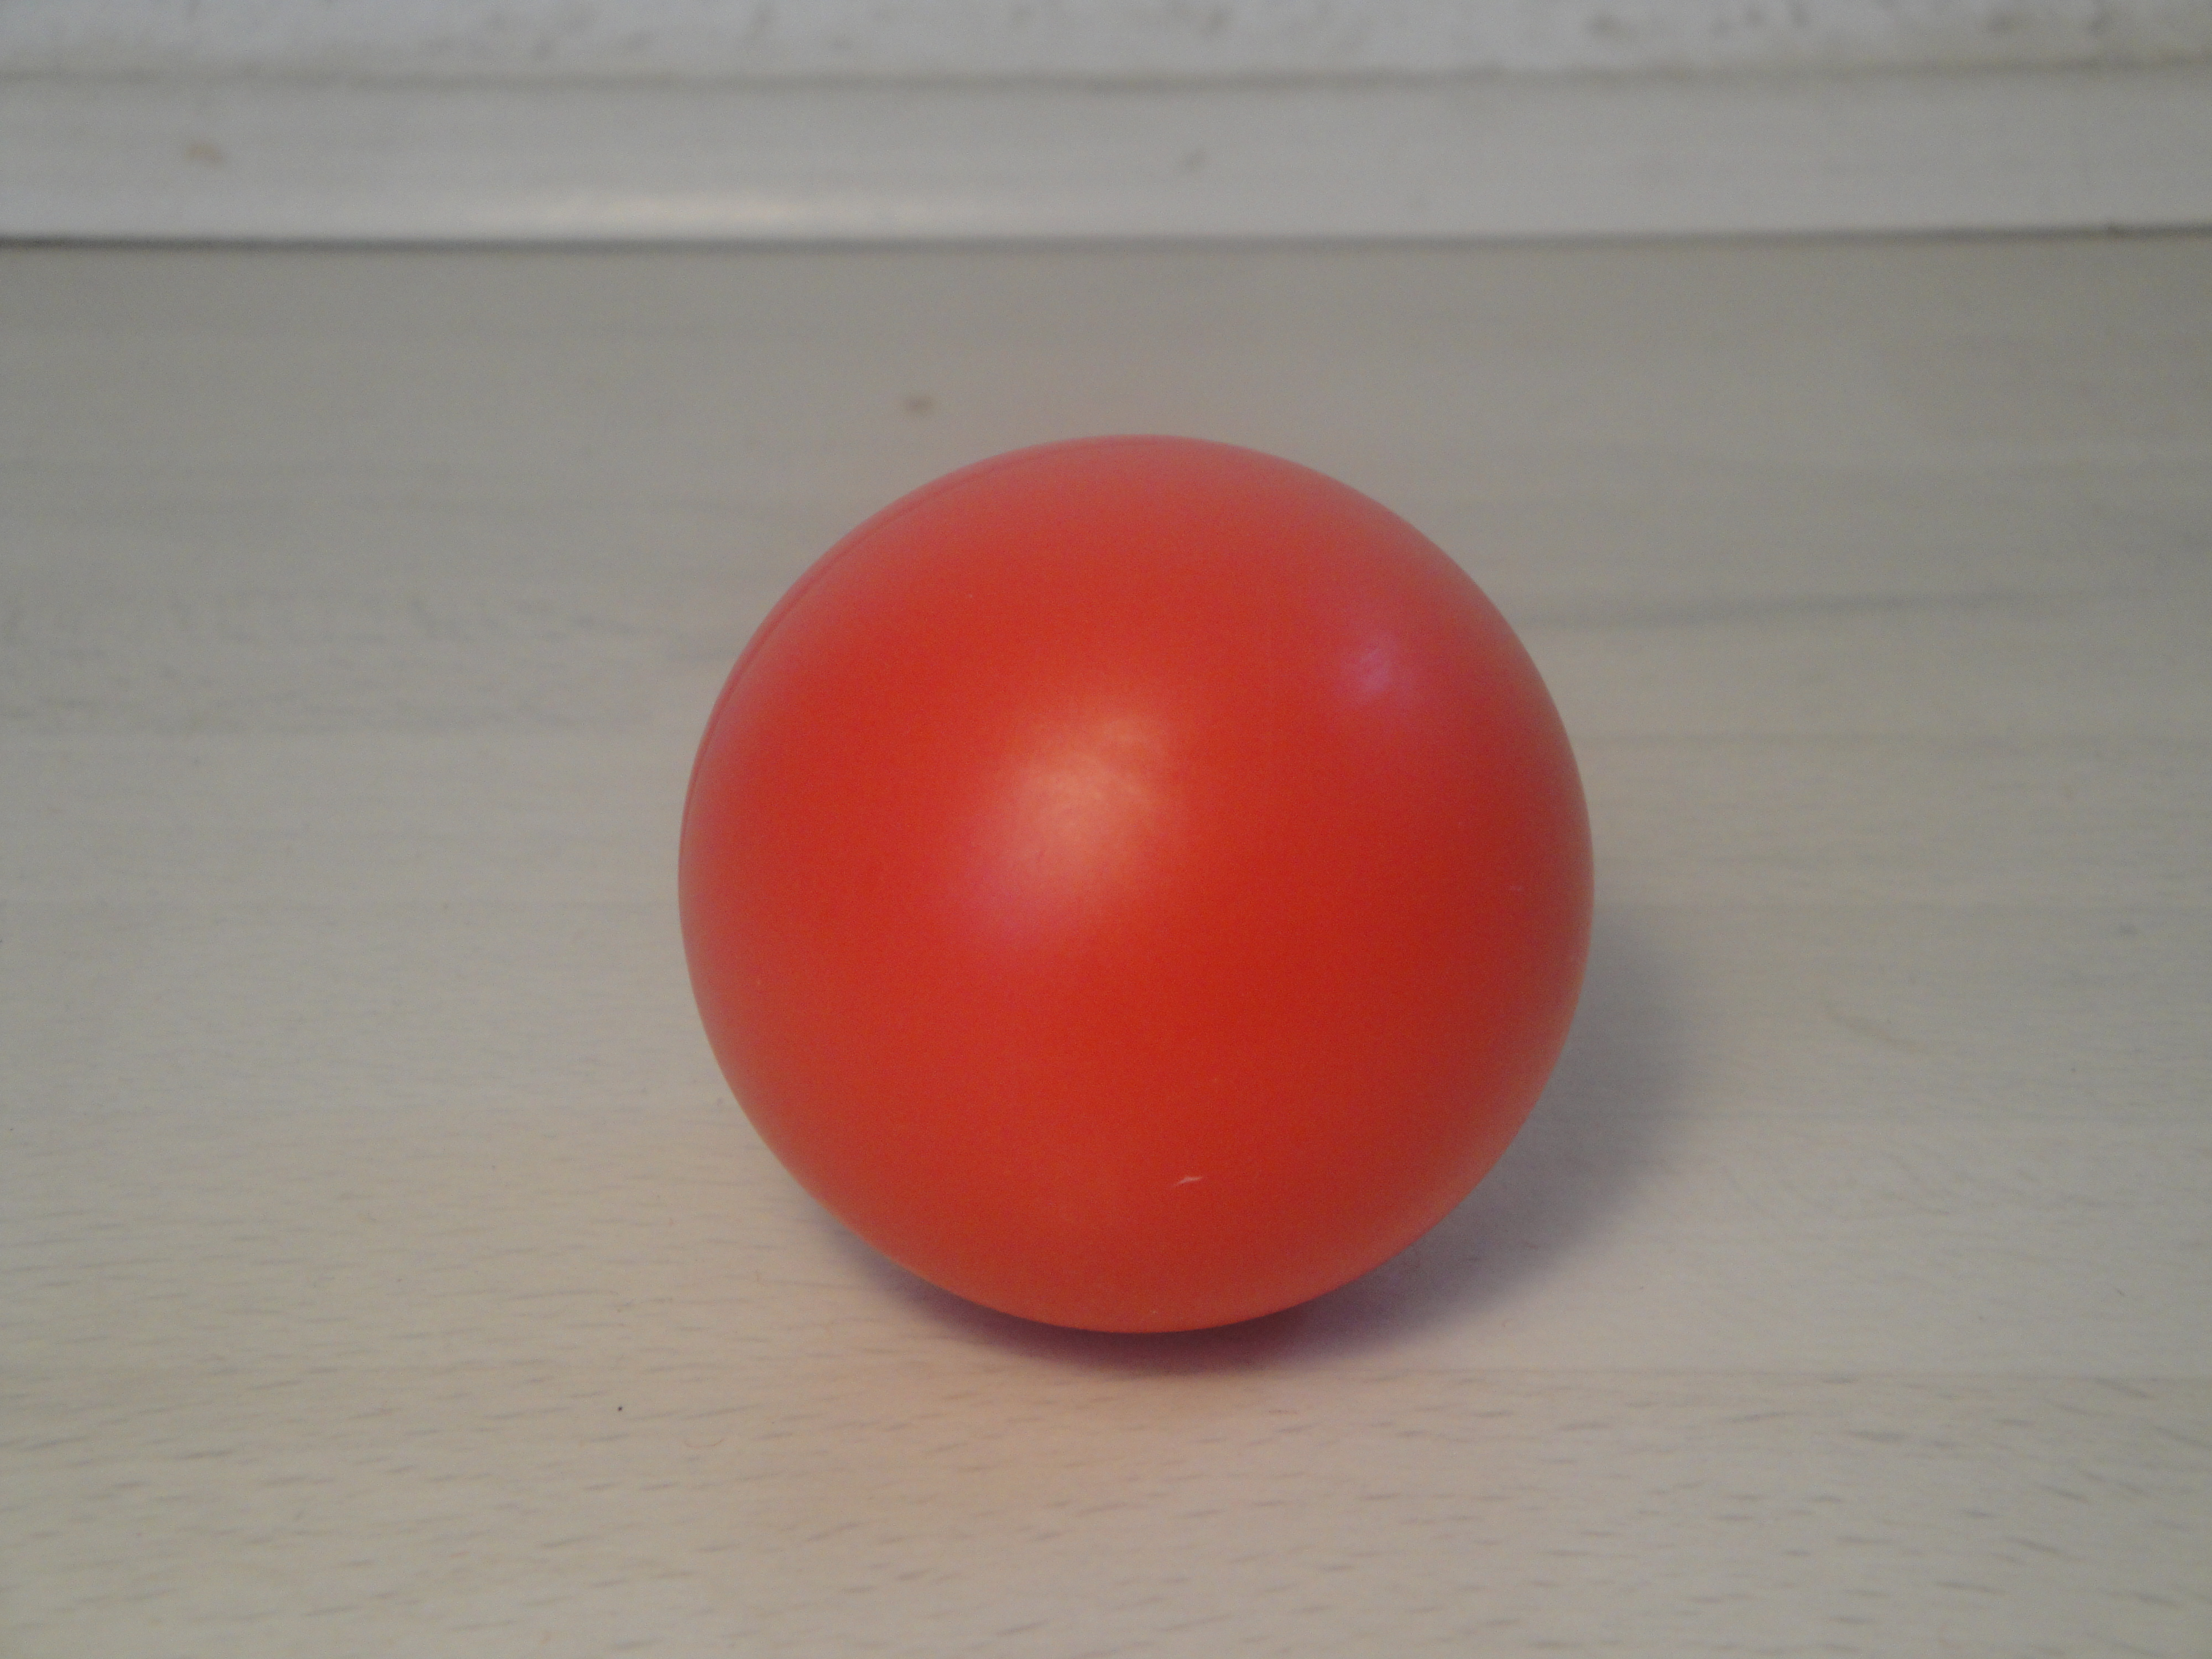
\includegraphics[width=\columnwidth]{img/ball1.jpg}%
            \caption{Die erste Version des Balls}%
            \label{img:ballv1}%
          \end{figure}
        \end{minipage}
        \hfill
        \begin{minipage}[t]{.49\textwidth}
          \begin{figure}[H]%
            \centering%
            \includegraphics[width=\columnwidth]{img/ball2.jpg}%
            \caption{Die finale Version des Balls}%
            \label{img:ballFinal}%
          \end{figure}
        \end{minipage}
      \end{center}

				
		%\subsection{Referenzen}\label{sec:Referenzen}
			%Es folgt eine Auflistung aller Referenzen zu den im Architekturentwurf erwähnten Fremdressourcen und verwendeten Dokumenten.
				%\printbibliography[heading=none]
		%	
\end{document}
